\documentclass[fleqn,12pt,openany]{book}

% These two need to be set before including scirun style package
\title{Meshing Pipeline User Guide}
\author{Brett Burton, Jess Tate, Jeroen Stinstra, Ayla Khan}

% INCLUDE SCI STYLE DOCUMENT
\usepackage{biomesh}
\usepackage{wrapfig}

\begin{document}

% CREATE TITLE PAGE --------------------------------------------------
\maketitle

% CHAPTERS ---------------------------------------------------------------

%%%%%%
\chapter{Overview}\label{overview}

This manual gives an overview of how to operate the BioMesh3D pipeline in its
current state. The BioMesh3D project aim to develop an easy to use 
program for generating quality meshes for the use in biological simulations.
The project's primary goal is to provide a solution that does not require much interaction of the
user and automatically generates a proper mesh.
\paragraph{}
Currently BioMesh3D is available is a prototype pipeline made up of a series of python scripts that are run sequentially that generates a mesh from a segmented volume.
Although the plan is to generate a complete user interface for the program, the user interface is not currently available.

%%%%%    
\chapter{Meshing pipeline stages}
\label{sec:tetgenflags}

\section{Introduction to Biomesh3D}
\label{sec:flags}

\paragraph{}
The Biomesh3D program simplifies the meshing pipeline by breaking it up into 
eight basic stages described below. Each stage fulfills specific tasks and 
produces specific outputs for later use downstream.  In order to run this 
pipeline a few software requirements are first essential components, 
namely Python and SCIRun.

\paragraph{}
Python is relatively simple to acquire, and SCIRun is 
an open source software package that can be downloaded from 
\url{http://www.sci.utah.edu/software.html}.

\paragraph{}
SCIRun software tools are required to run the BioMesh3D pipeline.
SCIRun can be built on OSX and Linux platforms using the {\bf build.sh} script that is included in the source distribution.
Use {\bf build.sh --help} for usage information.
Currently no other dependencies are required to run the meshing pipeline. 

\paragraph{}
Though BioMesh3D will soon have a more streamlined user interface, the current 
system requires a call to a python script. This python script is generated as 
part of the SCIRun distribution and can be found in the {\bf bin/FEMesher}
directory of SCIRun. The script that the user has to call is the {\bf BuildMesh.py }
script. This script will recursively call all the other scripts to complete the
mesh.

\paragraph{}
The {\bf BuildMesh.py} needs a description of the model it will mesh; this
model is defined in a second python script that initializes the meshing parameters.
This script is a user generated document that defines 
the path to the segmentation labelmap, the desired output directory, the names 
of materials to be meshed, and various other parameters discussed in the next section. 
Examples of these {\bf model\_config.py} can be found in the {\bf SCIRunData}
dataset in the folder {\bf FEMesher}.

\paragraph{}
In addition to the model configuration python script, there are 5 other flags 
that can be used directly after the {\bf BuildMesh.py} call. \\ \\
\emph{-h} provides a help menu with a brief description of each stage \\
\emph{-s} allows the user to define what stages to run (for example: ...BuildMesh.py -s2:5 will run stages 2 thru 5) \\
\emph{-i} executes the Biomesh3D pipeline interactively, pausing between each step and asking if the user would like to continue, while displaying the results within SCIRun. \\
\emph{-d} displays the output of key stages of the pipeline using SCIRun without running any of the meshing pipeline.  If used alone the files must already exist (that is the pipeline must have already been run) in order for this flag to work \\
\emph{-p} path to executables used in the pipeline [only required if the script cannot find the SCIRun programs in the default location].
\paragraph{}
With the exception of \emph{-h}, each of these flags can be used in tandem.  For example \emph{-s2:5 -i} will execute the pipeline interactively from stage 2 to stage 5.  Once each stage has been completed, the output will be displayed in SCIRun and the screen will prompt the user to continue.  Note: with \emph{-d} the command would need the files in stages 2 thru 5 to already exist.


\section{User Variables: model\_config.py}

\paragraph{}
The \verb+model_config.py+ file contains various variables that can be altered by the user, including:
\begin{itemize} 
  \item{\bf \verb+model_input_file+} - path to the input nrrd file
  \item{\bf \verb+model_output_path+} - path to the desired output directory
  \item{\bf \verb+mats+} - array from 0 to $n - 1$ where $n$ represents the number of materials
  \item{\bf \verb+mat_names+} - names the user wishes each material to be called (must be the same size as \verb+mats+)
 \item{\bf \verb+mat_radii+} - radius of tightening during the tightening process (if set to 0 tightening will be skipped)
 \item{\bf \verb+refinement_levels+} - number of levels that the medial axis will use
 \item{\bf \verb+max_sizing_field+} - sets a cap on sizing field.  The smaller the number the more dense the final mesh
 \item{\bf \verb+tetgen_joined_vol_flags+} - sets parameter flags for tetgen in generating the final mesh
 \item{\bf \verb+num_particles_iters+} - defines the number of iterations the particle system will execute
 \item{\bf \verb+max_procs+} - set the maximum number of processes run by the particle system
\end{itemize} 


\section{Initializer: BuildMesh.py}

\paragraph{}
{\bf BuildMesh.py} initiates the entire pipeline.  
It receives the command line flags \emph{-h, -s, -i, -d, -p} or, by default, 
runs the entire meshing pipeline if no flags are set.
Once these preliminary decisions are made, this script calls each of the following stages in order.

\section{Stage 1: MakeSolo.py}

\paragraph{}
MakeSolo.py first accepts the nrrd file defined in the \verb+model_cofig.py+ 
file and pads it with 0 in all dimensions.
The newly padded nrrd is unoriented and a transformation matrix is extracted for use in the final 
stage of the pipeline (in order to realign the final data with the original data).
Each material is then isolated and a separate nrrd file created for 
each material that is tightened (if \verb+mat_radii+ $\neq 0$ in the \verb+model_config.py+ 
file) and set aside for the next stage.   \\ \\
Output files are:

\begin{itemize}

\item{\emph{original-nrrd-name}\verb+_unorient.nrrd+}
\item{\emph{original-nrrd-name}\verb+_transform.tf+}
\item{\emph{material}\verb+.solo.nrrd+}
\item{\emph{material}\verb+.tight.nrrd+}
\item{\emph{material}\verb+.lut.raw+}
\item{\emph{material}\verb+.lut.nrrd+}
\item{\verb+medial_axis_param_file.txt+}
\item{\verb+make-solo-nrrd-runtime.txt+}

\end{itemize}

This stage does not display anything when the \emph{-d} flag is active.

\section{Stage 2: ComputeMaterialBoundary.py}

\paragraph{}
The material boundary is computed from the tightened nrrd files from the previous 
stage.
These files are converted to SCIRun fld files before their respective isosurfaces are extracted. \\ \\

Output files are:
\begin{itemize}

\item{\emph{material}\verb+_isosurface.ts.fld+}
\item{\emph{material}\verb+.tight.fld+}
\item{\verb+isosurface-all.ts.fld+}
\item{\verb+compute-material-boundary-runtime.txt+}

\end{itemize}

This stage displays the isosurfaces of all materials together when the \emph{-d} 
flag is active.  SCIRun users can view individual materials by adjusting which 
field is called in the ReadField module's user interface.

\section{Stage 3: ComputeMaterialMedialAxis.py}

\paragraph{}
Both the speed and the quality of the meshing pipeline are critically dependent 
on the quality (accuracy AND consistency) of the medial axis computation.  We 
have implemented a medial axis algorithm that extracts the medial axis by way 
of point cloud approximation.  The current method produces a point cloud over 
the entire volume and computes which points are closest to the medial axis.  
These points are then used to produce another homogeneously spaced point cloud 
in the region of each previously computed medial axis point where it is again 
checked for closeness to the medial axis.  This process iterates through a user-specified number of  
levels, each time honing in closer to the desired medial axis.  Due to the 
number of levels and the amount of point cloud particles produced, this stage 
can take a long time.  \\ \\

Output files are:
\begin{itemize}

\item{\emph{material}\verb+_ma.ptcl+}
\item{\emph{material}\verb+_ma.pc.fld+}
\item{\verb+ma-all.pc.fld+}
\item{\verb+compute-material-medial-axis-runtime.txt+}

\end{itemize}

This stage displays the medial axis points of each material within the 
isosurfaces of each material together when the \emph{-d} flag is active.  
SCIRun users can view individual materials by adjusting which field is 
called in the ReadField module's user interface.

\section{Stage 4: ComputeSizingField.py}

\paragraph{}
The medial axis points previously generated are used to generate a sizing field 
nrrd file for each material based on the distance of the medial axis to the 
isosurface of the material.  Also, a zero-crossing algorithm is used to isolate 
the boundary of each material generated in the MakeSolo.py script. \\ \\

Output files are:
\begin{itemize}

\item{\emph{material}\verb+_crossing.nrrd+}    
\item{\emph{material}\verb+_lfs.nrrd+}
\item{\emph{material}\verb+_sf_init.nrrd+}
\item{\emph{material}\verb+_sf.nrrd+}
\item{\verb+compute-sizing-field-runtime.txt+}

\end{itemize}

This stage displays the sizing field and associated grid of only one material 
at a time when the \emph{-d} flag is active.  SCIRun users can change which 
material they are looking at by adjusting which field is called in the 
ReadField module's user interface.

\section{Stage 5: GenerateSeeds.py}

\paragraph{}
Junctions where materials meet are determined and seed points are randomly 
placed along these junctions.  A dual junction (where two materials meet) 
creates a surface, the filename has a \emph{d} in front of it followed by the 
two material labels.  Triple junctions create lines represented by \emph{t} and 
the three material labels involved, and quadruple junctions make points 
(\emph{q} followed by four material labels).  \\ \\

Output files are:
\begin{itemize}

\item{\verb+generate-seeds-runtime.txt+} 
\item{\emph{seeds/}}
\subitem{\verb+d01_seed.pc.fld+}
\subitem{\verb+d01_seed.ptcl+}
\subitem{\verb+etc...+}
\subitem{\verb+t012_seed.pc.fld+ \emph{if there are triple interfaces}}
\subitem{\verb+t012_seed.ptcl+}
\subitem{\verb+etc...+}
\subitem{\verb+q0123_seed.pc.fld+ \emph{if there are quad interfaces}}
\subitem{\verb+q0123_seed.ptcl+}
\subitem{\verb+etc...+}
\subitem{\verb+seeds-all.pc.fld+}

\end{itemize}

This stage does not display anything when the \emph{-d} flag is active.

\section{Stage 6: DistributeParticles.py}

\paragraph{}
Using the sizing field as an energy metric (the smaller the sizing field value, 
the less energy) the seeds that were randomly placed on the surface of the 
material adjust themselves to minimize energy.  In general, the closer a seed 
is with its neighbor, the more energy exists between them.  These particles 
will move away from each other in an attempt to minimize energy while still 
being forced to remain on the surface.  By moving they interact with other 
particles and move again in an attempt to minimize energy.  The sizing field 
determines the energy that each particle has as they adjust themselves into a 
state of lowest energy.  Once the amount of iterations specified in the 
\verb+model_config.py+ file are met, the algorithm quits.  \\ \\

Output files are:
\begin{itemize}

\item{\verb+distribute-particles-runtime.txt+}
\item{\verb+ops-output-#.txt+}
\item{\emph{input}\verb+_+\emph{seeds/}}
\subitem{\verb+d01_seed.pc.fld+}
\subitem{\verb+etc...+}
\item{\emph{junctions/}}
\subitem{\verb+psystem_input.txt+}
\subitem{\verb+particle_params.txt+}
\subitem{\verb+m1.txt+}
\subitem{\verb+particle_params.txt_#.pts+}
\subitem{\verb+particle_params.txt_#.ptcl+}
\subitem{\verb+particle_params.txt_#.pcv.fld+}
\subitem{\verb+particle_params.txt_#.pc.fld+}
\subitem{\verb+particle-all.pcv.fld+}
\subitem{\verb+particle-all.pc.fld+}

\end{itemize}

This stage displays the final position of all particles for each material 
together when the \emph{-d} flag is active.

\section{Stage 7: BuildMaterialInterfaceMesh.py}

\paragraph{}
Using the particle system points, surfaces are generated that share nodes. \\ \\

Output files are:
\begin{itemize}

\item{\verb+build-material-interface-mesh-runtime.txt+}
\item{\emph{junctions/}}
\subitem{\verb+particle-union.pts+}
\subitem{\verb+particle-union.node+}
\subitem{\verb+particle-union.m+}
\subitem{\verb+particle-union.ts.fld+}
\subitem{\verb+particle-union.1.node+}
\subitem{\verb+particle-union.1.face+}
\subitem{\verb+particle-union.1.ele+}
\subitem{\emph{material}\verb+.m+}
\subitem{\emph{material}\verb+.ts.fld+}

\end{itemize}

This stage does not display anything when the \emph{-d} flag is active.

\section{Stage 8: BuildVolumetricMesh.py}

\paragraph{}
Tetgen is used to create a volumetric mesh of each material and of the materials 
together as a joined field based on the surfaces produced in stage 7. \\ \\

Output files are:
\begin{itemize}

\item{\verb+build-volumetric-mesh-runtime.txt+}
\item{\emph{junctions/}}
\subitem{\verb+particle-union.tets-labeled_transformed.fld+}

\end{itemize}

This stage displays the tetrahedralized mesh of the entire material with an 
overlaid quality tet mesh that uses a scaled Jacobian measure when the 
\emph{-d} flag is active.


%%%%%%
\chapter{Limitations and known issues}
\label{chapter:limitations}

\begin{itemize} 
  \item{\bf Data will be node centered throughout pipeline} - Though data 
  can be node centered or element centered, the pipeline (which accepts both) 
  will ultimately node center all data; thus, a shift will be perpetuated in 
  any element centered data that is used.
  
%  \item{\bf The number of materials is limited to 9 domains } - No more %than 9
%  different domains (including the domain that surrounds the segmented %volume)
%  can be handled by the current system.
  
  \item{\bf Performance } - The current system has not yet been optimized and as
  a result the system may take a few days to render a mesh for a large dataset.
  For example on our system a typical torso segmentation (512 by 512 by 400) takes,
  on average, one week to run to completion.  Furthermore, significant hard drive
  space is required for these datasets (10 GB for said torso meshes).  
  Smaller datasets with only two materials should require much 
  less space (less than 1GB) and will be much quicker (less than a day).

 \item{\bf 3D Data only} - BioMesh3D does not compensate for data of other 
 dimensions.
 
 \item{\bf Thin segmentations produce inaccuracies} - Blood vessels and other thin,
   narrow (approx. 1 - 2 voxels thick) might be eliminated by the tightening algorithm.
   Tightening can be turned off by setting $mat\_radii = 0$ in the $model\_config.py$ file.
 
  \item{\bf Interactive mode over forwarded X11 connections} - SCIRun has been 
  known to crash when volume rendering over forwarded X11 connections, therefore
  we recommend against running BioMesh3D in interactive mode over an X11 connection.
  Instead run the pipeline automatically and copy the files to your local machine
  and run the pipeline in the -d mode, which only will do the visualizations and
  use all the precomputed files.
  
  \item{\bf Large data sets require more memory than is available} - A temporary, hard coded 
  fix has been implemented for relatively large datasets by multiplying the binning radius by 4.  
  This will be changed to allow for a more dynamic handling of method so that large data sets
  will automatically reduce the size of the binning radius and allow for proper memory 
  management.

\end{itemize} 


%%%%%%    
\chapter{Preparing data for meshing pipeline}
\label{chapter:prep}

\section{Segmentations with Seg3D}

\paragraph{}
Segmentations of many kinds of data can be done using Seg3D.  With this program 
domains can be identified and assigned values from images, such as various 
tissue types from an MRI scan.  Seg3D will read many formats of slice data such 
as a DICOM file and other formats generated by imaging scanners.  After 
segmenting each of the tissue types, Seg3D can then export the segmentation in 
nrrd format, which is used by BioMesh3D.  A brief demonstration of how to use 
Seg3D is included in the tooth example (Chapter ~\ref{chapter:tooth}), but for 
a more extensive explanation of the tools and capabilities of Seg3D, please 
see the Seg3D documentation. 


%%%%%%     
\chapter{Example dataset: Mickey}
\label{chapter:mickey}
\paragraph{}
To demonstrate the functionality of BioMesh3D, we will use a simple, 
low-resolution model.  This example will walk you through how to access the 
example data sets and use SCIRun to create a 3D Mickey model (head and ears of Mickey Mouse).  

\section{Example Data Sets}
\paragraph{}
To obtain the mickey data set, download the {\bf SCIRunData.zip} file from
{\em http://software.sci.utah.edu/}. The SCIRunData set can be found in the 
SCIRun4.2 file/data repository. All the example files are stored in the
{\em FEMesher} directory.

Select the mickey folder and download the two files 
(\emph{mickey-unorient.nrrd} and \emph{model}\verb+_+\emph{config.py} into the 
directory from which you would like to work.  The *.nrrd file is our data file 
that is to be meshed.  The \emph{model}\verb+_+\emph{config.py} file is a 
python script full of variables that the user is able to manipulate as described 
above in Chapter \ref{sec:tetgenflags}.

\paragraph{}
For BioMesh3D to work on your data set, the \emph{model}\verb+_+\emph{config.py} 
file must point to the mickey file as well as an output directory (it does not 
matter whether the output directory is the same as the input directory).  Open 
the \emph{model}\verb+_+\emph{config.py} file and point the 
'model\verb+_+input\verb+_+file' and 'model\verb+_+output\verb+_+path' 
variables at the proper paths. These paths can be relative to the \emph{model}\verb+_+\emph{config.py} file.
The default settings assume that the segmentation file is in the same directory
as the \emph{model}\verb+_+\emph{config.py} file.


\paragraph{}
Open a terminal from which you can run command line code.  Type the command 
described in the first section of Chapter \ref{sec:tetgenflags} (if you are 
already in the SCIRun directory, there is no need to include the path to your 
SCIRun directory).  The files will generate themselves as the program runs.  
If you would like to view the stages as they progress use the \emph{-i} flag.  
If you wish to only run certain stages is the \emph{-s} flag; however, if this 
is a fresh run, you will have to start from stage 1 in order to get any results.

\paragraph{}
The following results were obtained by using the following command:
From the SCIRun directory \\ \\
\emph{bin/BuildMesh.py} -i \\ \emph{$<$path-to-mickey$>$/Mickey/model}\verb+_+\emph{config.py}  \\ \\
\begin{figure}[h!]
\begin{center}
\scalebox{0.3}{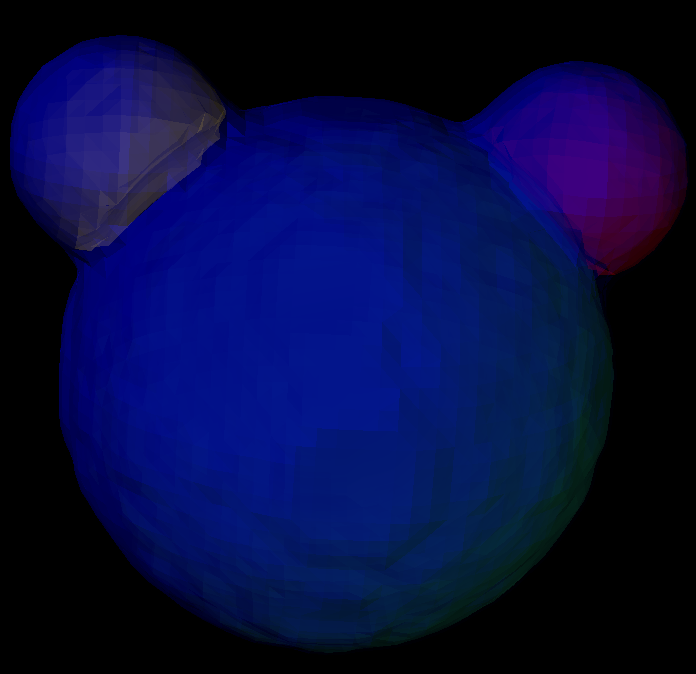
\includegraphics{BioMesh3DGuide_figures/MickeySurf.png}}
\end{center}
\caption{\label{fig:MickeySurf} Stage 2: Extract Material Surfaces - Isosurfaces of the three materials that make up mickey (head, left-ear, and right-ear)}
\end{figure} 

\begin{figure}[htp]
\begin{center}
\scalebox{0.3}{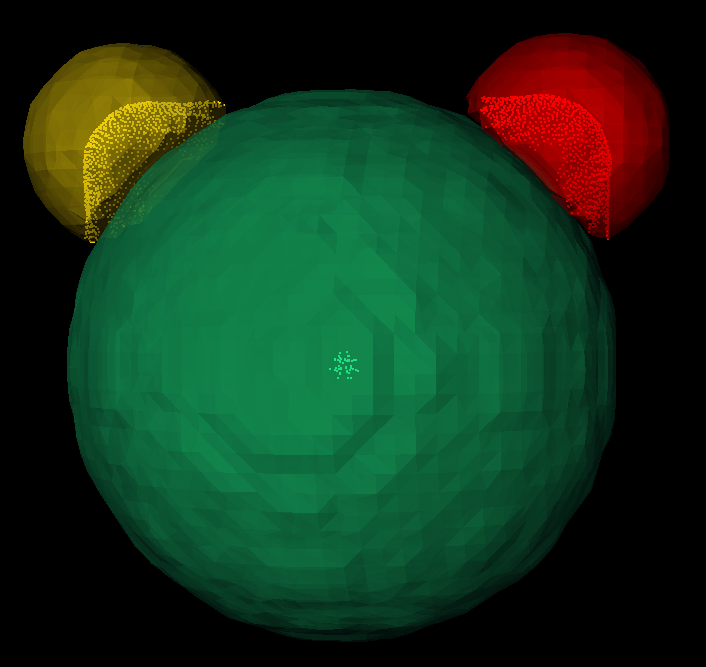
\includegraphics{BioMesh3DGuide_figures/MickeyMA.png}}
\end{center}
\caption{\label{fig:MickeyMA}Stage 3: Compute Medial Axis - Medial axis points of the mickey.}
\end{figure} 

\begin{figure}[htp]
\begin{center}
\scalebox{0.3}{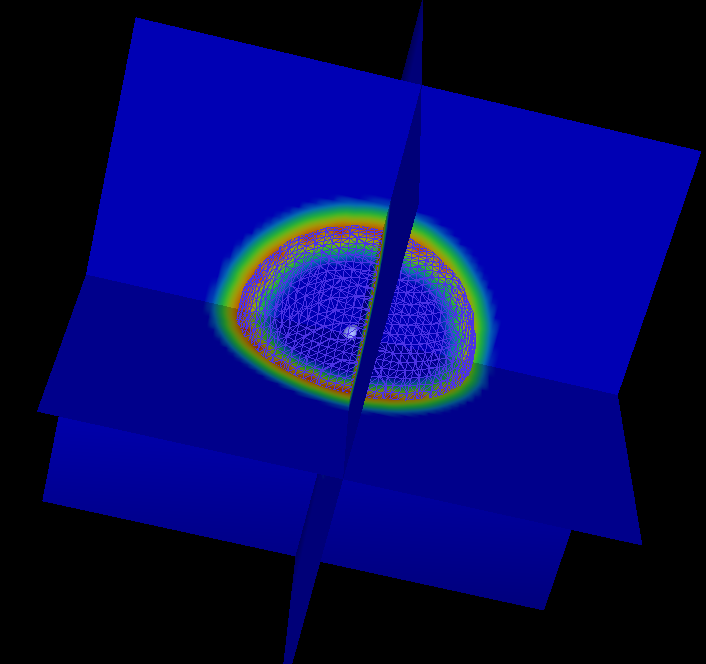
\includegraphics{BioMesh3DGuide_figures/MickeySF.png}}
\end{center}
\caption{\label{fig:MickeySF}Stage 4: Compute Sizing Field - Computed from the medial axis, the sizing field is a distance map from the medial axis points to the surface of the material.  Sizing field files are only shown one material at a time (this being the head).}
\end{figure} 

\begin{figure}[h!]
\begin{center}
\scalebox{0.3}{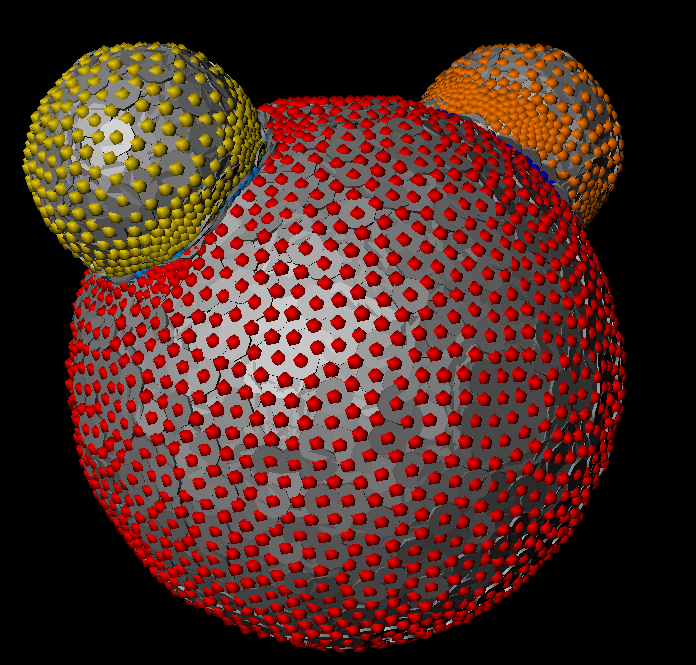
\includegraphics{BioMesh3DGuide_figures/MickeyPS.png}}
\end{center}
\caption{\label{fig:MickeyPS}Stage 6: Run Particle System - A high resolution particle system (that is when max\_sizing\_field and SIZING SCALE VAR values are low) will produce tightly packed particles such as these.}
\end{figure} 
Stage 7: Generate Surface Mesh (no visualization) \\ \\

\begin{figure}[h!]
\begin{center}
\scalebox{0.3}{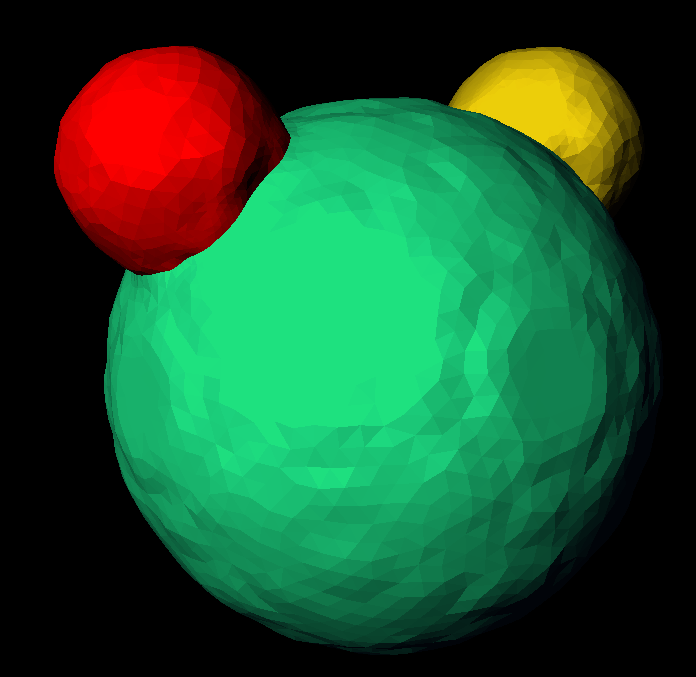
\includegraphics{BioMesh3DGuide_figures/MickeyMesh1.png}}
\scalebox{0.3}{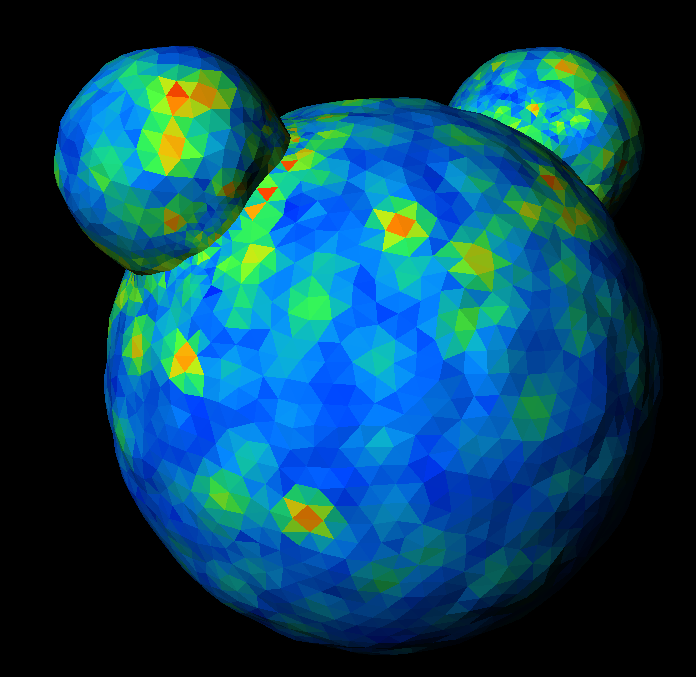
\includegraphics{BioMesh3DGuide_figures/MickeyMesh.png}}
\end{center}
\caption{\label{fig:MickeySurf}Stage 8: Generate Volume Mesh - Final mesh (left) and associated quality field (right).  Red tetrahedra are higher quality than blue.}
\end{figure} 
  


%%%%%%    
\chapter{Example dataset: Tooth}
\label{chapter:tooth}
\paragraph{}
This Example will walk you through the basics of generating a mesh from raw data. 
There are two basic steps: creating the segmentation and running the BioMesh3D 
script. The data file is available in the SCIRunData/FEMesher/tooth/volume-tooth/ 
directory.  Similarly, in the SCIRunData/FEMesher/tooth/ directory, there is a 
{\bf tooth.nrrd} file that is similar to the one that will be created in the 
tutorial in the following section.  Therefore, the first section of the tooth 
tutorial, wherein Seg3D is used to make a segmentation can be skipped. 
 However, Seg3D is a useful tool that is compatible with BioMesh3D and SCIRun, 
 so it is encouraged to use this tutorial or the tutorial provided for Seg3D to 
 become familiar with it if the user intends to make meshes from raw scan data.

\section{Creating a segmentation using Seg3D}

\paragraph{}
Open Seg3D and create a new project.  Under the `File' menu, choose `Import Layer From Single File ' and open $tooth.nhdr$ that was just downloaded or from the path mentioned above.  Import
the file as a 'Data Volume.'  A grayscale volume 
will appear.  Become familiar with the basic controls and navigation in Seg3D.  
Be sure to `save session' often as you segment to ensure that you do not lose 
any data.  For further instruction in the operation of Seg3D, please consult 
the Seg3D documentation.

\begin{figure}
\scalebox{0.34}{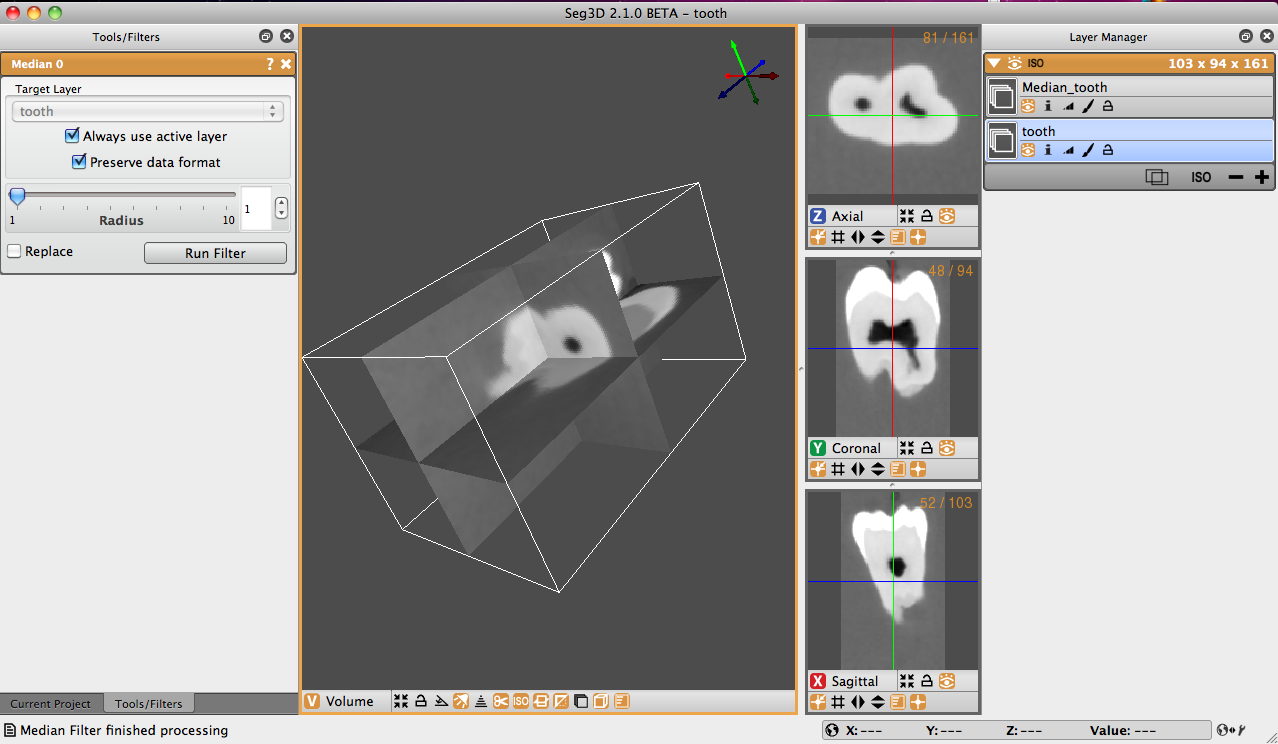
\includegraphics {BioMesh3DGuide_figures/tooth_filtered.png}}
\caption{\label{fig:tooth_filtered} Tooth volume after Median Filter.}
\end{figure} 
 
With the tooth volume loaded, perform a median filter on the data.  This filter 
will make it easier to perform segmentation tasks later.  This is done by 
clicking  `Median'  option under the `Data Filters' menu.  Leave the radius 
at 1 and press the Run Filter button.  Another layer will appear containing a 
blurrier but smoother tooth volume. Notice that the three main intensity 
regions of the tooth are more uniform (Figure ~\ref{fig:tooth_filtered}).  
we will label each of these three regions to be identified by BioMesh3D 
and other programs.

\begin{figure}
\scalebox{0.34}{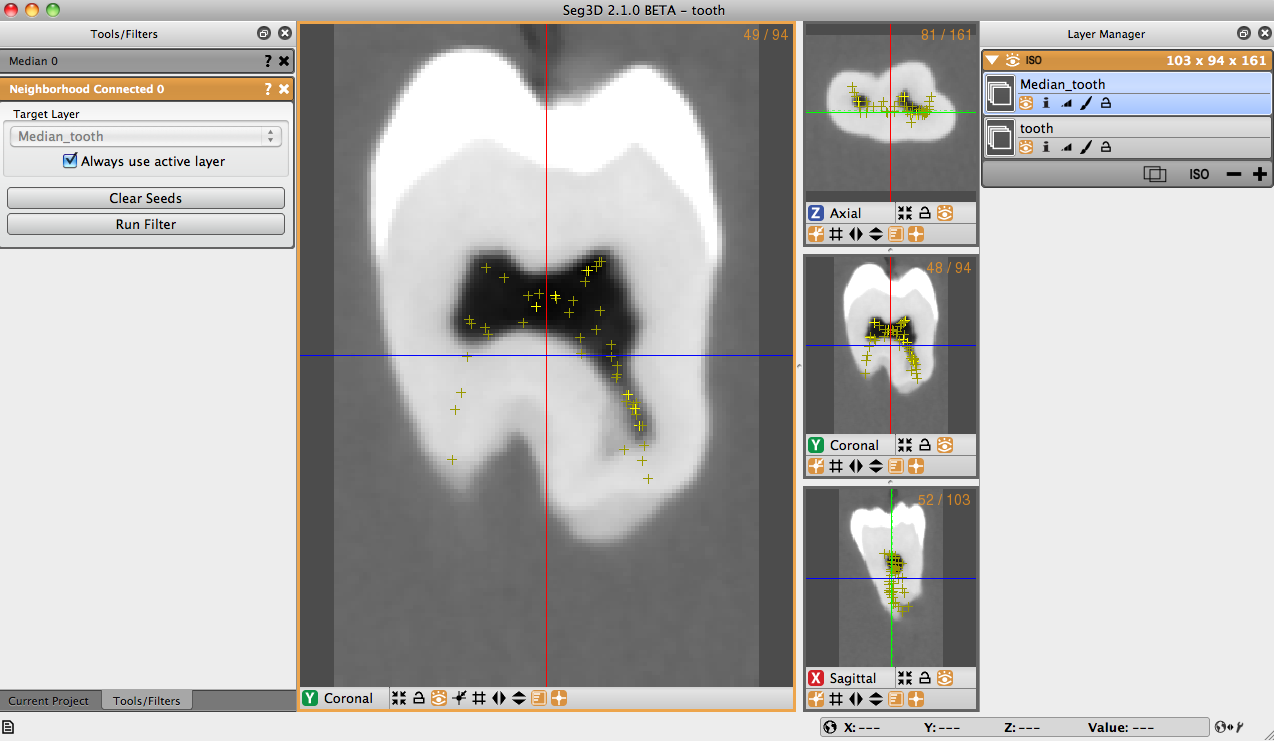
\includegraphics{BioMesh3DGuide_figures/tooth_seeds.png}}
\caption{\label{fig:tooth_seeds} Choosing the seed points.}
\end{figure} 

We will begin with the darkest region of the tooth.  Select 
`Neighborhood Connected' under the `Data Filters' menu.  This filter will 
use seed points to label bordering pixels of similar values.  To set the 
seeds, simply click on the dark region of the tooth 
(Figure ~\ref{fig:tooth_seeds}).  Set enough seed points that will encompass 
enough value range to get the area wanted.  Scroll through multiple slices using
the arrow keys while the cursor hoovers over the view you want to change, and then 
 set seeds on more than one slice.

\begin{figure}
\scalebox{0.34}{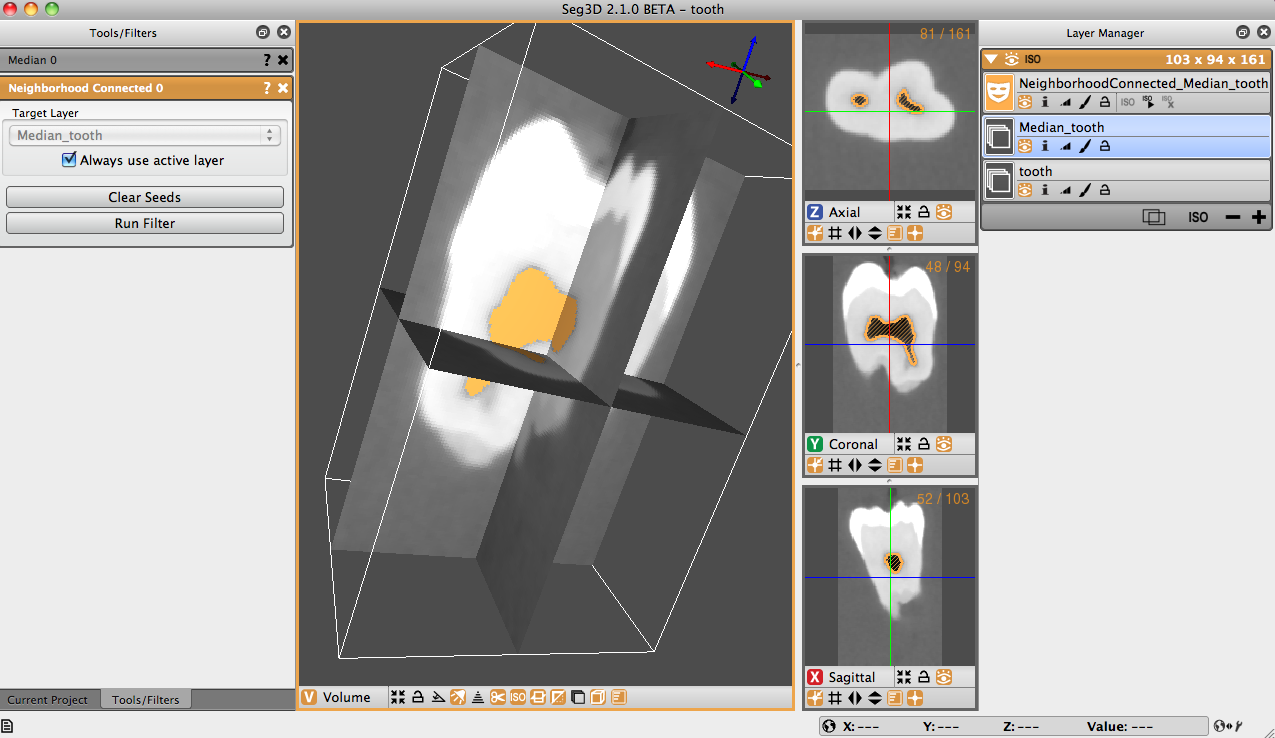
\includegraphics{BioMesh3DGuide_figures/tooth_afterneighborhood.png}}
\caption{\label{fig:tooth_firstone} Darkest region labeled.}
\end{figure}

 This will probably require many seed points and some experimenting.  Keep 
 running the filter and adding more seed points as needed (the seed points will 
 be saved until they are cleared) until the entire darkest area is covered by 
 the label (Figure ~\ref{fig:tooth_firstone}).  Delete all the extra labels 
 that were generated while you practiced.  Now you have one of the regions finished.  Rename
 this label to 'DarkRegion'.

\begin{figure}
\scalebox{0.34}{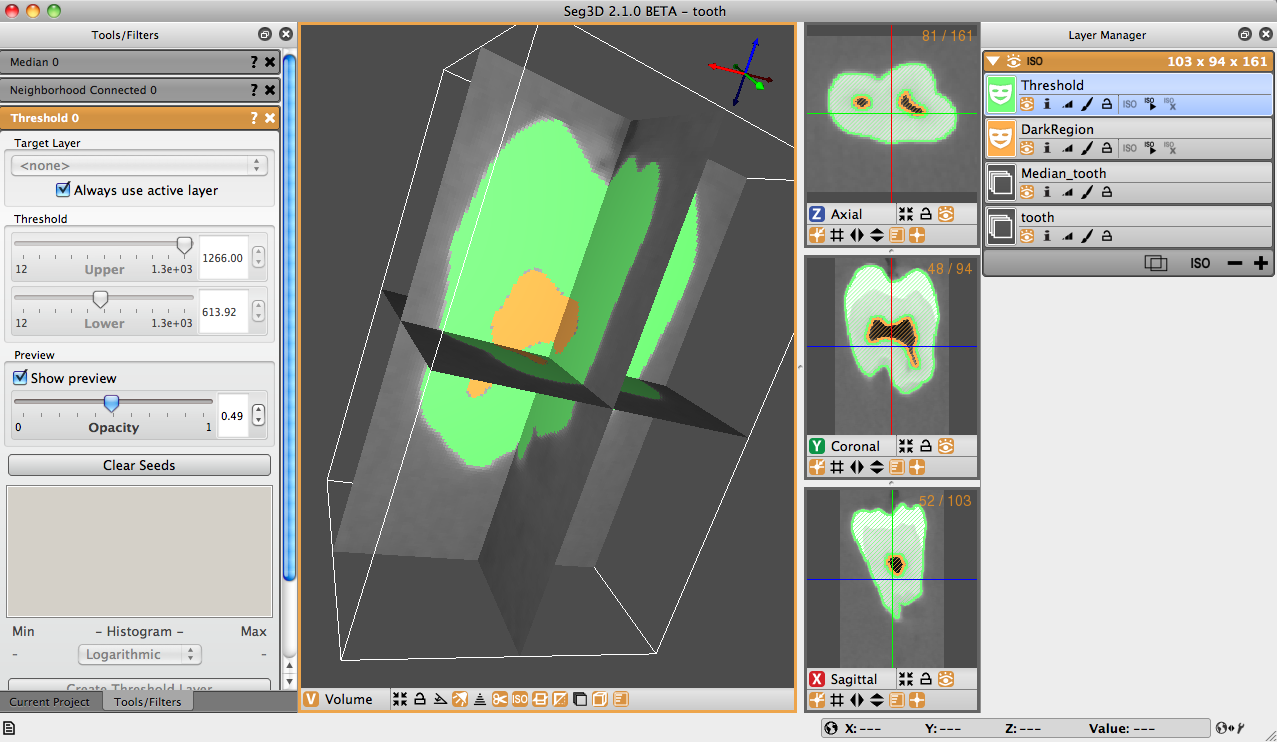
\includegraphics{BioMesh3DGuide_figures/tooth_threshold.png}}
\caption{\label{fig:tooth_threshold} Selecting the tooth using the threshold tool.}
\end{figure} 

For the second region, select `Threshold' under the `Tools' menu.  
This tool will label all the pixels in the volume that have a value between the 
set thresholds.  The thresholds can be set by seed points, but there are also 
slider bars to select values to label.  Choose threshold values that will label 
the entire tooth volume except the darkest regions 
(Figure ~\ref{fig:tooth_threshold}).  Make sure that the area selected by the 
threshold filter overlaps the label that you made for the darkest regions
slightly.  Press the 'Run Filter' button.  Rename the layer to 'Threshold'.

\begin{figure}
\scalebox{0.34}{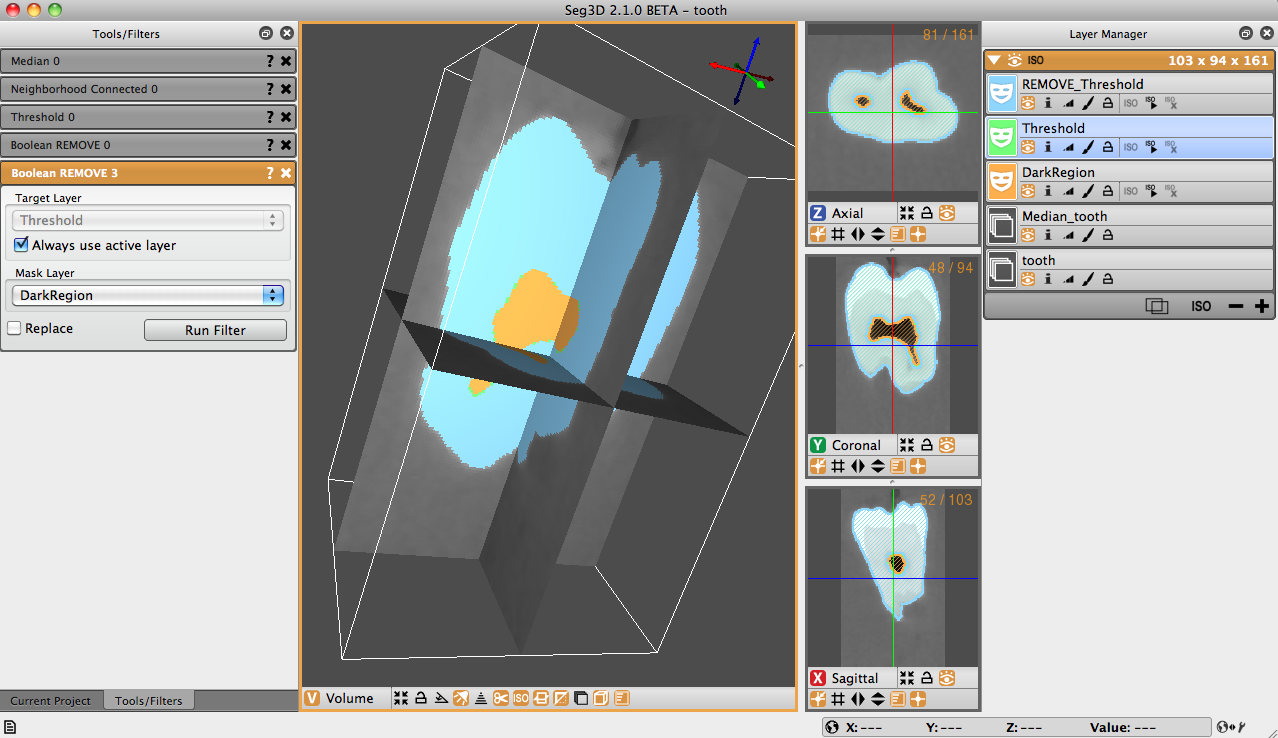
\includegraphics{BioMesh3DGuide_figures/tooth_remove_during.png}}
\caption{\label{fig:tooth_remove_during} Removing the overlapping regions using 'Boolean Remove'.}
\end{figure} 

To get rid of the overlap, choose the `BooleanRemove' 
tool from the `Mask Filters' menu.  Set the Target Layer to 'Threshold' or the layer you just made. Set Mask Layer to 'DarkRegion' or the layer you made from the darkest region.  Run this filter by clicking 'Run Filter'.

(Figure ~\ref{fig:tooth_remove_during}).  A new label should appear that does
not overlap called 'REMOVE\_ Threshold' if you have renamed the labels as described above.  

\begin{figure}
\scalebox{0.34}{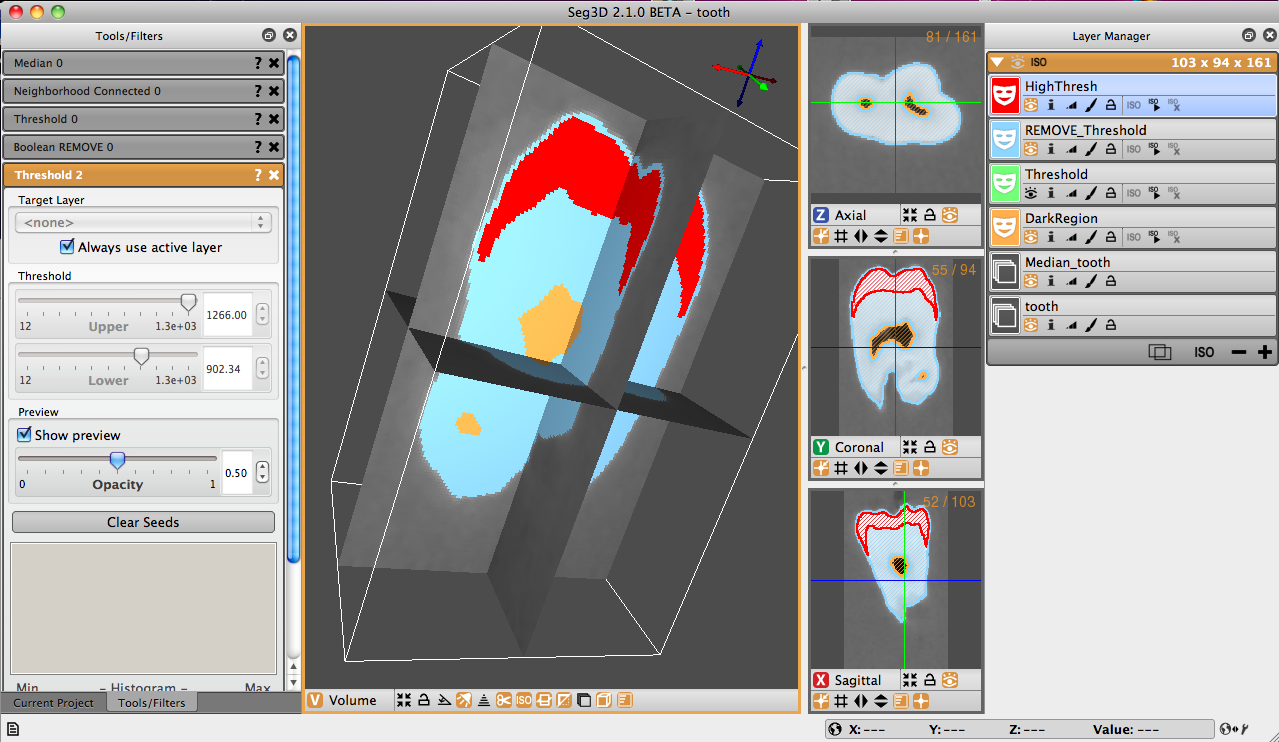
\includegraphics{BioMesh3DGuide_figures/tooth_paint.png}}
\caption{\label{fig:tooth_paint}  Using the paint brush tool to modify the labels to map areas not selected by the filter.}
\end{figure} 

Open the `Threshold' tool once again.  Now set the threshold to select the 
highest intensity  region in the tooth.  Make sure that it is as big a 
threshold as possible without getting stray pixels.  The label for the whitest 
region is meant to extend to the top of the tooth so that there is none of the 
previously made layers above it.  If this is not the case, then open the 'Paint Brush'
from the 'Tools' menu and set the 
bigger label as 'Mask Constraint 1'.  It will probably be called 'REMOVE\_ Threshold'
under the `Edit' menu.  Now simply paint the remaining pixels to extend the white region 
(Figure ~\ref{fig:tooth_paint}).  The mask will help make painting easier, 
but this still has to be done slice by slice, so the painting can be skipped.  
It just makes the mesh look nicer.  Rename the layer to 'HighThresh'.

\begin{figure}
\scalebox{0.34}{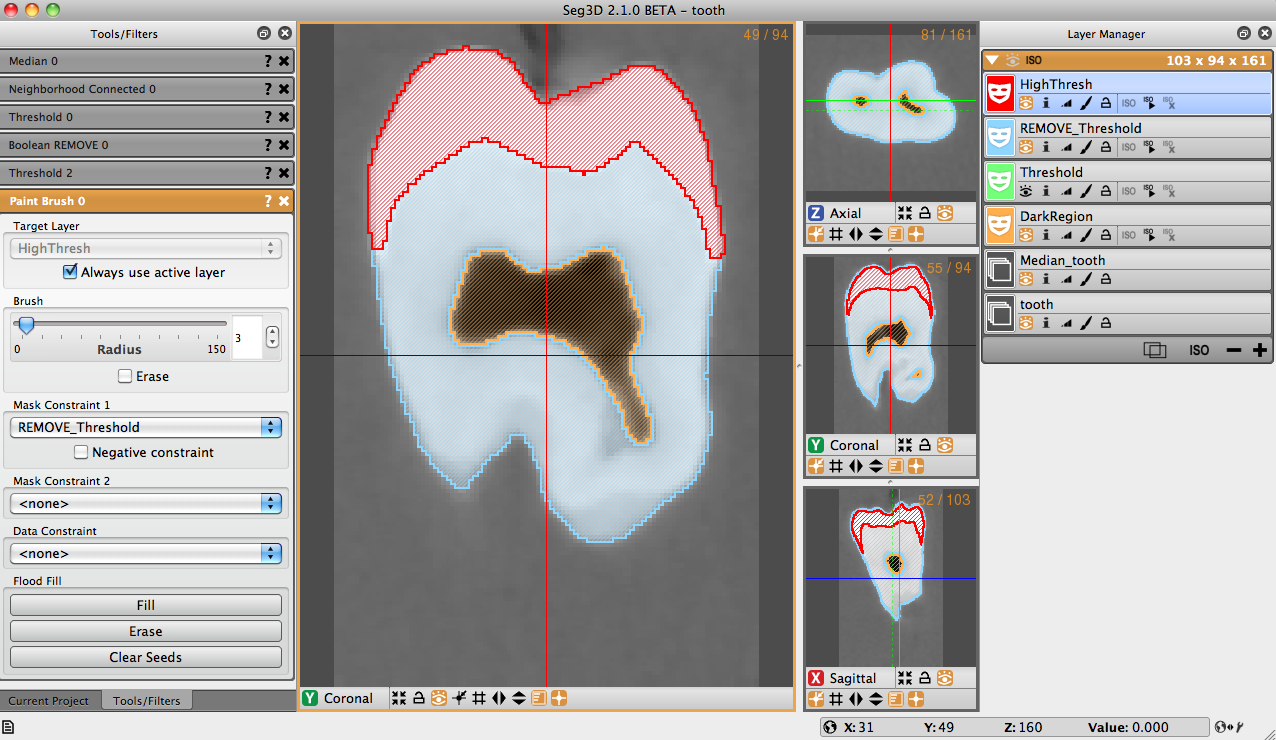
\includegraphics{BioMesh3DGuide_figures/tooth_3types.png}}
\caption{\label{fig:tooth_3types} Final three regions segmented, ready for export.}
\end{figure} 

Once the label for the whitest region is fully selected, use the `BooleanRemove' tool again.  
Select the Target Layer as 'REMOVE\_ Threshold' and the Mask Layer as 'High Threshold'.  Also
select the 'Replace' box before clicking the 'Run Filter' button.  Rename REMOVE\_ Threshold to MiddleThresh.  There should be three labels for each of 
the obvious regions in the tooth (Figure ~\ref{fig:tooth_3types}).  They should 
not over lap or contain any gaps between them.  If there are, the mesh can still 
be run through BioMesh3D, but it won't be as pretty.  Once the three regions of 
the tooth are correctly labeled `Export Segmentation' under the `File' menu.  
Uncheck the group box and then select the three of the correct labels, HighThresh, MiddleThresh, and DarkRegion.  Then click Continue.  Give the output .nrrd a name like 'tooth' and verify that the labels are numbered as you would like and then click Done.
This is the file that will be used in subsequent steps.  Once the segmentation 
is exported from Seg3D, it can run through BioMesh3D.


 

\section{Running BioMesh3D}

\paragraph{}
The actual running of BioMesh3D does not require much work on your part, just 
start it and let the computer crunch through it.  The $model\_config.py$ setup 
file needs to be edited to fit your machine and project.  There are examples 
of this configuration file in the directory \textbf{bin/FEMesher}.
\newline
 

It is suggested that a $model\_config.py$ file be made for each dataset run 
in BioMesh3D.

There are several variables in the $model\_config.py$ that need to be set.  

The variables are as follows:

\begin{itemize}
	\item model\_input\_file: The path for the mesh that will be input into the pipeline, in our case the segmentation of the tooth (.../tooth.nrrd).
	\item model\_output\_path: The path for the output files that will be generated by BioMesh3D (.../tooth).
	\item mats: The mask or data values of the materials in the input fields.  In the case of our tooth segmentation, there are four materials:  the three different regions that we segmented, and the air around it.  These are all assigned a value by Seg3D beginning with 0.  With the tooth file that we are using, we will assign this variable (0,1,2,3).
	\item mat\_names: The names of the materials labeled in the segmentation.  Each material labeled in the mats variable needs to have unique name.  For simplicity, we will assign the mat\_names variable (`air', `mat1', `mat2', `mat3').
	\item mat\_radii: This variable is a parameter for the tightening that is performed in the second stage to make the meshes smoother.  To turn off tightening, such as for very thin (one or two voxels thick) meshes, set this parameter to 0. For the tooth file that we are using, we can leave the default value 0.8.  
	\item refinement\_levels: This will modify the generation and refinement of the medial axis points.  A higher value will allow for more refinement, and thus medial axis points will be closer together. This variable can be set higher if the segmentation is very small or narrow.
	\item max\_sizing\_field: Modifies the sizing field algorithm.  A lower number generates more final elements on the tetrahedral mesh.
	\item SIZING\_SCALE\_VAR: A lower number generates more final elements on the tetrahedral mesh.
	\item num\_particle\_iters: The number of iterations used in the particle system in stage 6 of the pipeline.  The particle system generates equally spaced points to generate tetrahedra.  For the tooth.nrrd file, set the variable to 500.
	\item tetgen\_joined\_vol\_flags: This variable is similar to the previous, except it applies to the tetrahedral models generated for all the materials combined into a single file.  The flags available in this option are the same as the previous variable.  It can be left as ``zpAAqa10".
	\item max\_procs: Caps the number of processes used by the particle system (stage 6).
\end{itemize}

Once the $model\_config.py$ file is set to your liking, you're ready to run the 
script to execute the pipeline.  The command to run the script has three parts: 
the path to the BuildMesh.py script and the path to the $model\_config.py$ file.  

Open a terminal window, and type the following as one command:\\

[...]{\bf bin/BuildMesh.py}  [{\it flags}] [...] {\bf /model\_config.py}\\ \\

To see the other flags available for BioMesh3D, please refer to Section~\ref{sec:flags}.

The script may take a while to finish, depending on the system you are using and 
the size of the dataset.  The tooth file will probably take between twenty 
minutes and an hour.  If it takes longer, then it is likely that the script 
crashed and needs to be restarted.  Look for error messages as the script runs and 
check the parameters in the $model\_config.py$ file accordingly.  

Once BioMesh3D confirms that it is complete, look in the junctions directory 
in the defined output directory.  There will be a file named particle-union.tets-labeled\_transformed.fld, which is a tetrahedral mesh labeled with the values given for each material in the $model\_config.py$.


\section{BioMesh3D Output}
\label{sec:output}

The following images are the output of each of the display stages (using the the -d flag).  To see these images, it is recommended that the entire script run to completion, then re-execute the script with the \emph{-id} flags.  This will show the displays without re-executing the script.


\begin{figure}
\begin{center}
\scalebox{0.3}{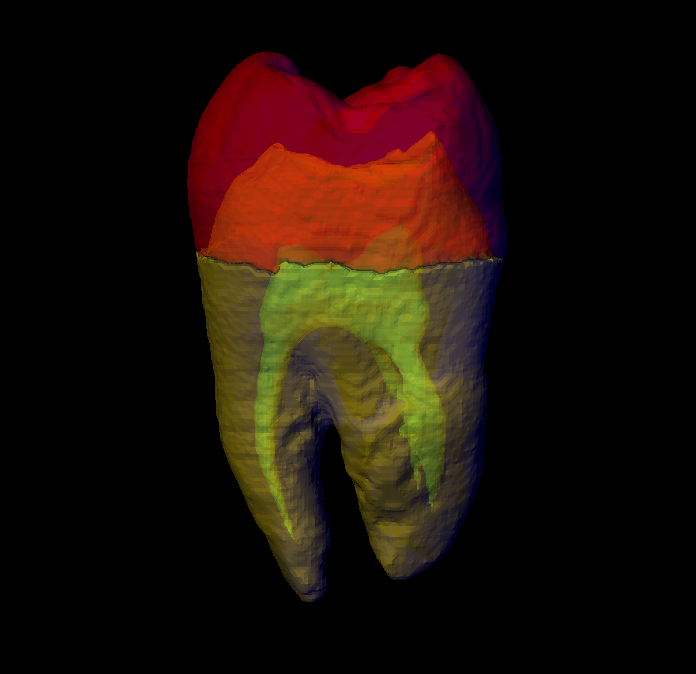
\includegraphics{BioMesh3DGuide_figures/stage1.png}}
\end{center}
\caption{\label{fig:tooth_stage1} The output of Stage 2.  This is the isosurface of each of the material type.}
\end{figure} 


\begin{figure}
\begin{center}
\scalebox{0.3}{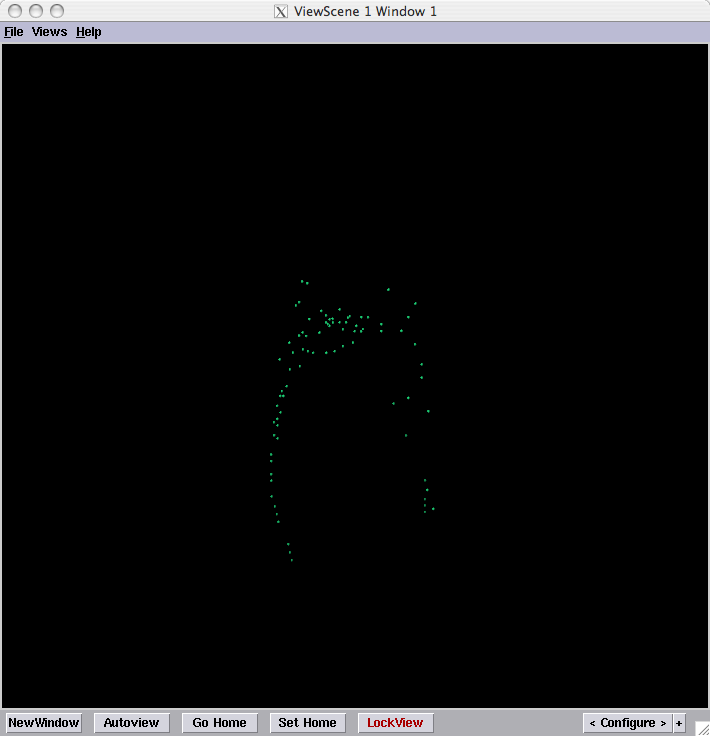
\includegraphics{BioMesh3DGuide_figures/stage2-2.png}}
\end{center}
\caption{\label{fig:tooth_stage2-2} The output of Stage 3.  These points are the medial axis points.  The medial axis points are generated for each material, but only the first material is shown by default.}
\end{figure} 


\begin{figure}
\begin{center}
\scalebox{0.3}{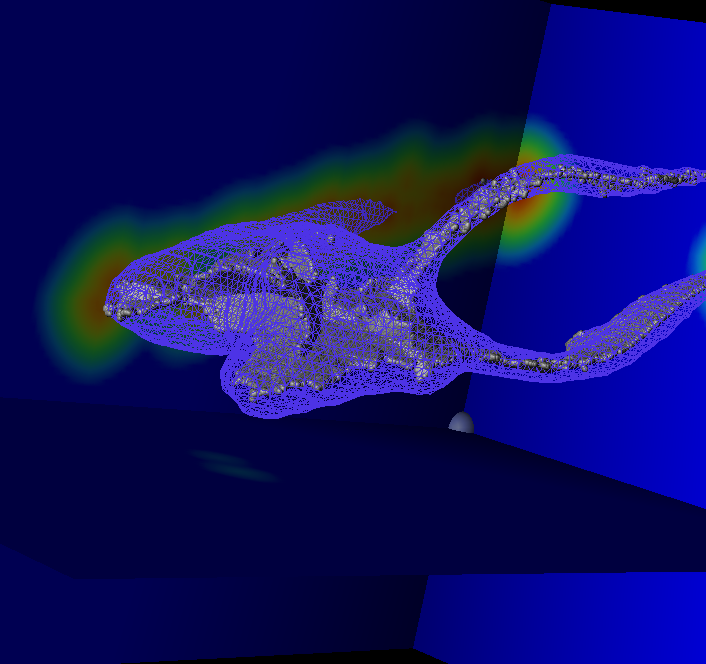
\includegraphics{BioMesh3DGuide_figures/stage3.png}}
\end{center}
\caption{\label{fig:tooth_stage3} The output of Stage 4.  This shows the sizing field and the medial axis points meshed together.}
\end{figure} 

\begin{figure}
\begin{center}
\scalebox{0.3}{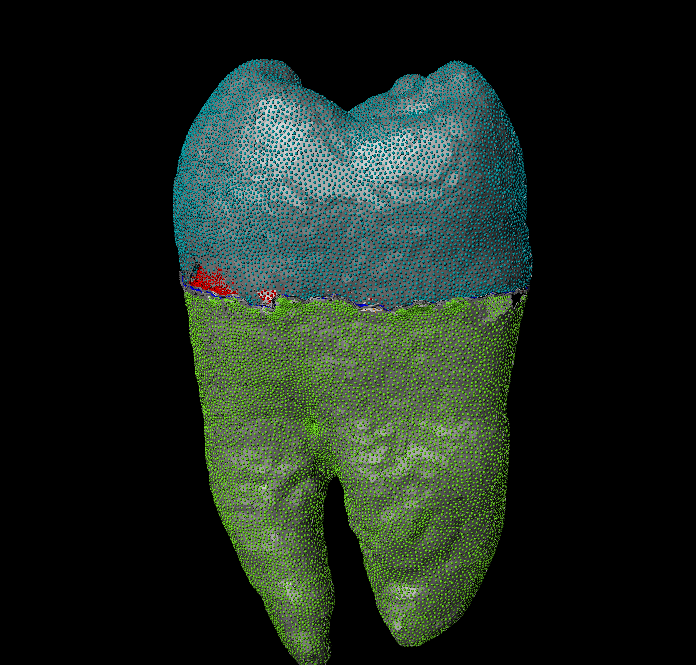
\includegraphics{BioMesh3DGuide_figures/stage4.png}}
\end{center}
\caption{\label{fig:tooth_stage4} The output of Stage 6.  The particles shown are the points used to generate the tetrahedral meshes.}
\end{figure} 

\begin{figure}
\begin{center}
\scalebox{0.3}{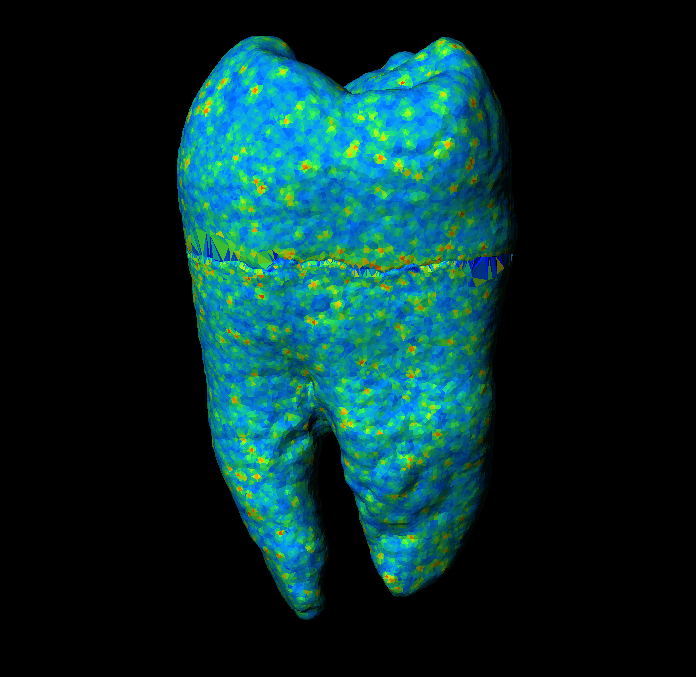
\includegraphics{BioMesh3DGuide_figures/stage5.png}}
\end{center}
\caption{\label{fig:tooth_stage5} The final mesh generated by BioMesh3D.  The color map represents the mesh quality of the tetrahedra.  Red is high and blue is low.}
\end{figure} 



\end{document}
